\documentclass[10pt,twocolumn,letterpaper]{article}

\usepackage{cvpr}
\usepackage{times}
\usepackage{epsfig}
\usepackage{graphicx}
\usepackage{amsmath}
\usepackage{amssymb}

\usepackage[utf8]{inputenc}
\usepackage[english]{babel}
\usepackage[T1]{fontenc}

\usepackage{subcaption}
\usepackage[draft,inline,nomargin]{fixme} % Enable fixme-notes.
\usepackage{units}

\makeatletter
\newcommand*\rel@kern[1]{\kern#1\dimexpr\macc@kerna}
\newcommand*\widebar[1]{%
  \begingroup
  \def\mathaccent##1##2{%
    \rel@kern{0.8}%
    \overline{\rel@kern{-0.8}\macc@nucleus\rel@kern{0.2}}%
    \rel@kern{-0.2}%
  }%
  \macc@depth\@ne
  \let\math@bgroup\@empty \let\math@egroup\macc@set@skewchar
  \mathsurround\z@ \frozen@everymath{\mathgroup\macc@group\relax}%
  \macc@set@skewchar\relax
  \let\mathaccentV\macc@nested@a
  \macc@nested@a\relax111{#1}%
  \endgroup
}
\makeatother

\graphicspath{{pictures/}}

% Include other packages here, before hyperref.

% If you comment hyperref and then uncomment it, you should delete
% egpaper.aux before re-running latex.  (Or just hit 'q' on the first latex
% run, let it finish, and you should be clear).
\usepackage[pagebackref=true,breaklinks=true,letterpaper=true,colorlinks,bookmarks=false]{hyperref}

%\cvprfinalcopy % *** Uncomment this line for the final submission

\def\cvprPaperID{****} % *** Enter the CVPR Paper ID here
\def\httilde{\mbox{\tt\raisebox{-.5ex}{\symbol{126}}}}

% Pages are numbered in submission mode, and unnumbered in camera-ready
\ifcvprfinal\pagestyle{empty}\fi
\begin{document}

%%%%%%%%% TITLE
\title{Tri-modal Human Body Segmentation}

\author{Chris Bahnsen, Andreas Møgelmose, Thomas B. Moeslund\\
Aalborg University\\
Sofiendalsvej 11, 9200 Aalborg SV, Denmark\\
{\tt\small \{cb, am, tbm\}@create.aau.dk}
% For a paper whose authors are all at the same institution,
% omit the following lines up until the closing ``}''.
% Additional authors and addresses can be added with ``\and'',
% just like the second author.
% To save space, use either the email address or home page, not both
}

\maketitle
%\thispagestyle{empty}

%%%%%%%%% ABSTRACT
\begin{abstract}
   The ABSTRACT is to be in fully-justified italicized text, at the top
   of the left-hand column, below the author and affiliation
   information. Use the word ``Abstract'' as the title, in 12-point
   Times, boldface type, centered relative to the column, initially
   capitalized. The abstract is to be in 10-point, single-spaced type.
   Leave two blank lines after the Abstract, then begin the main text.
   Look at previous CVPR abstracts to get a feel for style and length.
\end{abstract}

%%%%%%%%% BODY TEXT
\section{Introduction}
\label{sec:introduction}

Segmentation of people in images is still nowadays a very challenging and tough problem for the computer vision community due to the great diversity of poses that they can adopt and their variable appearance. Difficulties also arise from changes in lighting conditions and complex and cluttered backgrounds. The general idea of human body segmentation is to assign a label to every pixel or group of pixels in an image such that pixels with the same label share certain visual characteristics which entitles them to be considered as part of a human. These type of problems are commonly referred to as labeling problems. Despite extensive research done so far, some constraints have still to be taken into account and one often has to make assumptions about the scenario where the segmentation task is to be applied, such as static versus moving camera, indoor versus outdoor, and so on. Ideally, it should be tackled in an automatic fashion rather than relying on user intervention, which makes such task even more challenging. 

There exist a wide range of possible applications for people segmentation such as surveillance, content-based image retrieval, activity recognition, patient caregiving or human-computer interaction among others. Such task is also often related to pose estimation problems, since it can be carried out efficiently once the person is detected and segmented in an image. Furthermore, it can facilitate the task of photo edition, chroma-keying or video compression. Hence, human body segmentation can be considered as an important preprocessing step for other tasks.

State of the art methods that tackle the human segmentation task mostly use color images recorded by RGB cameras as the main cue for further analysis, although they present several widely known intrinsic problems such as intensity similarities between background and foreground. More recently, the release of RGB-Depth devices such as Microsoft\textsuperscript\textregistered Kinect\textsuperscript\texttrademark , a cheap multi-sensor device based on structured light technology, has allowed the community to use RGB images along with per-pixel depth information, often called depth maps, thus increasing the robustness of the methods. Besides, this device has helped boost research in human pose and behavior analysis.

In this context, we propose adding a third modality: thermal imagery got from thermal infrared cameras, thus complementing other information sources and making easier the segmentation task. Although thermal cameras are relatively expensive devices, their market price is lowering substantially every year --as it happens with other sensory devices. Besides, they can capture data similar to standard color cameras but without having illumination problems, that is why infrared cameras are becoming popular in surveillance scenarios and other similar applications. To do so, we introduce a novel tri-modal database provided by researchers from Aalborg University in Denmark and Universitat de Barcelona. Such database contains people acting in three different video sequences, consisting of more than 2,000 frames each one, in which three different subjects appear and interact with objects performing diverse actions such as reading, working with a laptop, speaking on the phone, etc. There may be more than one subject appearing in scene. The dataset comes along with an algorithm that performs the registration among modalities. 

In addition, we present a baseline methodology to automatically segment people in video sequences in indoor scenarios with a fixed camera. With all the available modalities, important features will be extracted using different state of the art descriptors, which are used to learn a probabilistic model so as to predict the image regions belonging to people. We will compare results from applying segmentation to the different modalities separately to results obtained by fusing features from all modalities.

To the best of our knowledge, this is the first dataset and work that combines color, depth and thermal modalities to perform the people segmentation task in videos, aiming to bring further benefits towards developing more robust solutions.

The remainder of this dissertation is organized as follows. Section \ref{sec:relatedwork} reviews the different approaches for human body segmentation that appear in the recent literature. Section \ref{sec:proposedbaseline} introduces and exhaustively explains the proposed baseline methodology, which will be experimentally evaluated in Section \ref{sec:evaluation}. Finally, Section \ref{sec:conclusions} concludes this dissertation.

\section{Acquisition}
\label{sec:setup}
The tri-modal data stream is recorded using a Microsoft Kinect for XBOX 360 capturing the RGB and depth image streams, and an AXIS Q1922 thermal camera. The resolution of the imagery is fixed at 640x480 pixels. As seen in Figure \ref{fig:camerasetup}, the cameras are vertically aligned in order to reduce perspective distortion. 

\begin{figure}[htpb]
	\centering
		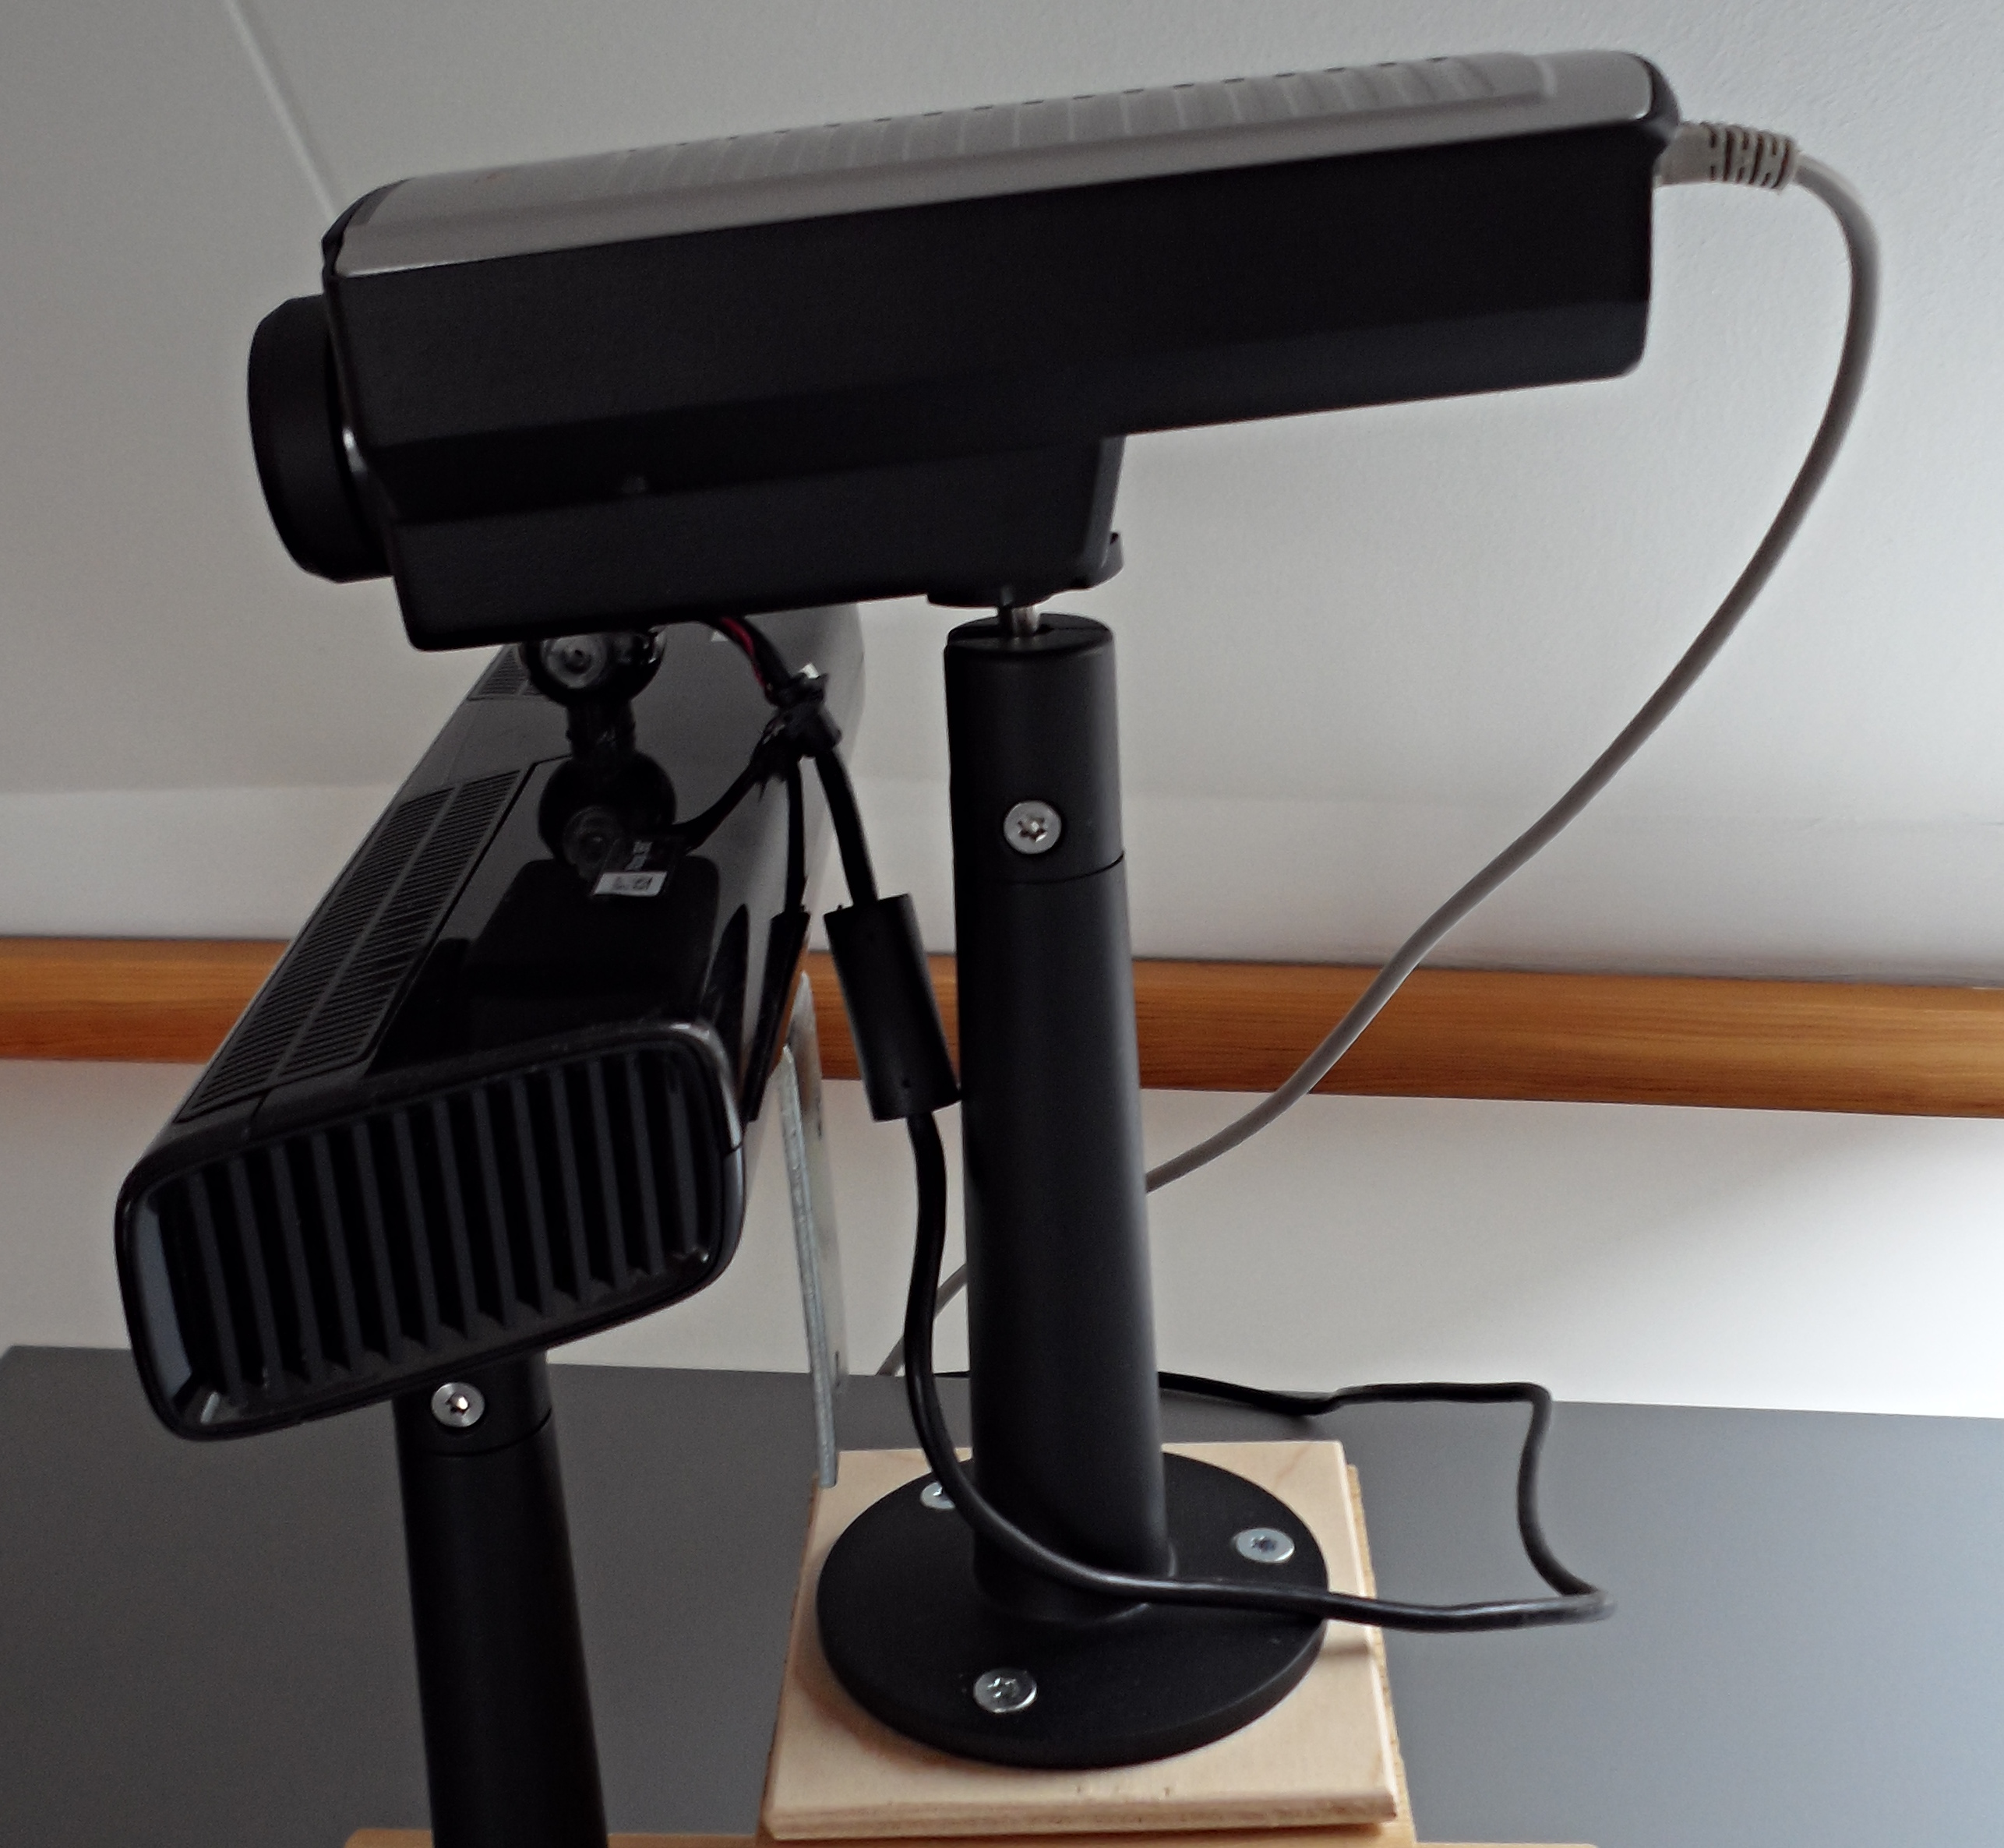
\includegraphics[width=0.25\textwidth]{pictures/camerasetup.jpg}
	\caption{Camera configuration. The RGB and thermal sensor are vertically aligned.}
	\label{fig:camerasetup}
\end{figure}

The image streams are captured using custom recording software that invokes the Kinect for Windows and AXIS Media Control SDKs. The integration of the two SDKs enables the cameras to be calibrated against the same system clock, which enables the post-capture temporal alignment of the image streams. Both cameras are able to record at 30 FPS. However, the data set is recorded at 15 FPS due to performance constraints of the recording software. 

\subsection{Multi-modal calibration}
The calibration of the thermal and RGB cameras have been accomplished using a thermal-visible calibration device inspired by \cite{vidas2012mask}. The calibration device consists of two parts; an A3-sized 10 mm polystyrene foam board is used as a backdrop and an equally sized board with cut-out squares is used as the checkerboard. Before using the calibration device, the backdrop is heated and the checkerboard plate is kept at room temperature, thus keeping a suitable thermal contrast when joined, as is seen from Figure \ref{fig:calibrationDevice}. %The depth sensor of the Kinect is factory calibrated and a subsequent calibration is thus not needed.
Using the Camera Calibration Toolbox of \cite{bouguet2004camera}, we are able to extract corresponding points in the thermal and RGB modalities. The sets of corresponding points are used to undistort both image streams and for the subsequent registration of the modalities. 

\begin{figure}[htpb]
\centering
\begin{subfigure}[b]{0.48\columnwidth}
	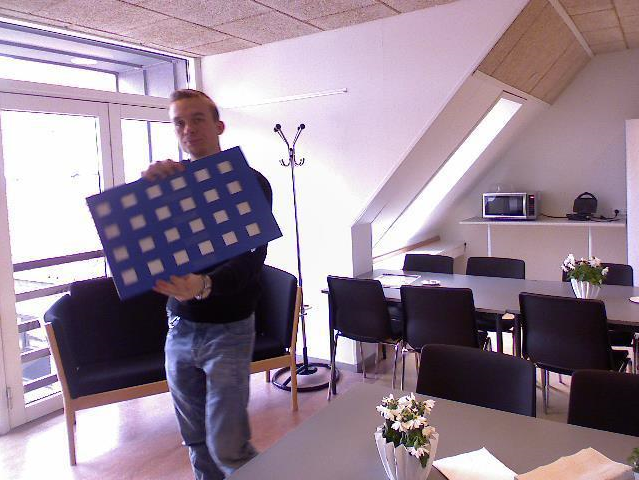
\includegraphics[width=\columnwidth]{RGB00064.png}%
	\caption{}
\end{subfigure}
\begin{subfigure}[b]{0.48\columnwidth}
	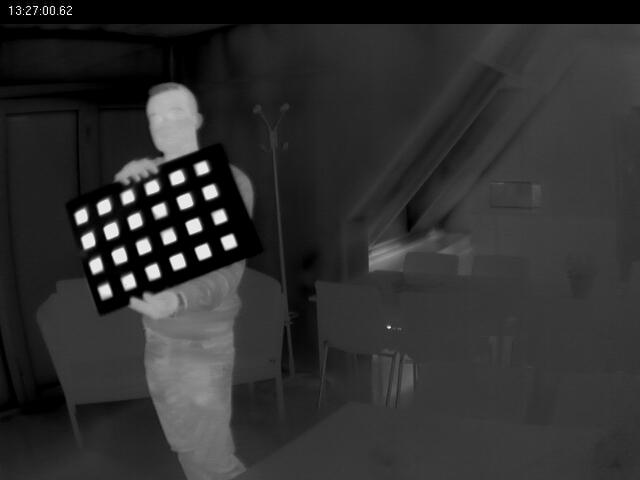
\includegraphics[width=\columnwidth]{T00064.jpg}%
	\caption{}%
\end{subfigure}
\begin{subfigure}[b]{0.48\columnwidth}
	\includegraphics[width=\columnwidth]{plane1.pdf}%
	\caption{}
\end{subfigure}
\begin{subfigure}[b]{0.48\columnwidth}
	\includegraphics[width=\columnwidth]{plane3.pdf}%
	\caption{}%
\end{subfigure}
\caption{The calibration device as seen by the (a) RGB and (b) thermal camera. The corresponding points in world coordinates is seen in (c) and the plane, which induces an homography, is overlayed in (d). Noise in the depth information accounts for the outliers in (c) and (d).}
\label{fig:calibrationDevice}
\end{figure}


\section{Registration}
\label{sec:registration}
The depth sensor of the Kinect is factory registered to the RGB camera and a point-to-point correspondence is obtained from the SDK. The registration is static and might thus be saved in two look-up-tables for $\text{RGB} \Leftrightarrow \text{depth}$. %The LUT shows to be inaccurate at positions where the Kinect cannot estimate the depth. This inaccuracy can be solved, however, by smoothing the LUT by a linear polynomial. 

The registration from $\text{RGB} \Rightarrow \text{thermal}$, $\mathbf{x} \Rightarrow \mathbf{x}'$, is handled using a weighted set of multiple homographies based on the approximate distance in space to the view that the homography represents. By using multiple homographies, we are allowed to compensate for parallax at different depths. However, the spatial dependency of the registration implies that no fixed, global registration or look-up-table is possible, thus inducing a unique mapping for each pixel at different depths.

Homographies relating RGB and thermal modalities are generated from minimum 50 views of the calibration device scattered throughout each scene. One view of the calibration device induces 96 sets of corresponding points in the RGB and thermal modality (Figure \ref{fig:calibrationDevice}c) from which a homography is computed using a RANSAC-based method. The acquired homography and the registration it establishes is only accurate for points on the plane that is spanned by the particular view of the calibration device. To register an arbitrary point of the scene, $\mathbf{x} \Rightarrow \mathbf{x}'$, the eight closest homographies are weighted according to this scheme:

\begin{enumerate}
	\item For all $J$ views of the calibration device, calculate the 3D centre of the $K$ extracted points in the image plane:
\begin{equation}
\widebar{\mathbf{X}}_{j} = \frac{\sum_{k=1}^K \mathbf{X}_{k_j}}{K} = \frac{\sum_{k=1}^K \mathbf{P}^+ \mathbf{x}_{k_j}}{K}
\end{equation}
The depth coordinate of $\mathbf{X}$ is estimated from the registered point in the depth image. $\mathbf{P}^+$ is the pseudoinverse of the projection matrix.
\item Find the distance from the reprojected point $\mathbf{X}$ to the homography centres:
\begin{equation}
\omega(j) = \lvert \mathbf{X} - \widebar{\mathbf{X}}_{j} \rvert
\end{equation}
\item Centre a 3D coordinate system around the reprojected point $\mathbf{X}$ and find $\min \omega(j)$ for each octant of the coordinate system. Set $\omega(j) = 0$ for all other weights. Normalize the weights:
\begin{equation}
\omega^*(j) = \frac{\omega(j)}{\sum_{j=1}^J \omega(j)}
\end{equation}
\item Perform the registration $\mathbf{x} \Rightarrow \mathbf{x}'$ by using a weighted sum of the homographies:
\begin{equation}
\mathbf{x}' = \sum_{j=1}^J \omega^*(j) \ \mathbf{H}_j \mathbf{x}
\end{equation}
Where $\mathbf{H}_j$ is the homography induced by the j\textsuperscript{th} view of the calibration device.
\end{enumerate}

%The spatial dependency of the registration algorithm implies that no fixed registration or look-up-table is possible. Thus, in order to register an image, one must know the spatial properties of each pixel, including depth information. 
For registering thermal points, the absence of depth information means that points are reprojected at a fixed distance, inducing parallax for points at different depths. Thus, the registration framework may be written:
\begin{align}
\text{depth} \Leftrightarrow \text{RGB} \Rightarrow \text{thermal}
\label{eq:mappingDiagram}
\end{align}

The accuracy of the registration of $\text{RGB} \Rightarrow \text{thermal}$ is mainly dependent on: 
\begin{enumerate}
	\item The distance in space to the nearest homography. %In theory, the error is proportional to the distance to the plane spanned by the homography; in practice, however, the Euclidean distance to the centre is a better estimate. 
	\item The synchronization of thermal and RGB cameras. At 15 FPS, the maximal theoretical temporal misalignment between frames is thus 34 ms. 
	\item The accuracy of the depth estimate.
\end{enumerate}
An example of the registration is seen from Figure \ref{fig:registeredImagery}. 

\begin{figure}[htpb]
\centering
\begin{subfigure}[b]{0.48\columnwidth}
	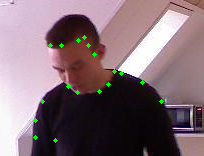
\includegraphics[width=\columnwidth]{RGBregistered.png}%
	\caption{}%
	\label{}%
\end{subfigure}
\begin{subfigure}[b]{0.48\columnwidth}
	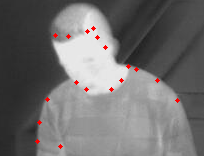
\includegraphics[width=\columnwidth]{Thermalregistered.png}%
	\caption{}%
	\label{}%
\end{subfigure}
\caption{Example of $\text{RGB (a)} \Rightarrow \text{thermal (b)}$ registration.}
\label{fig:registeredImagery}
\end{figure}



\section{Evaluation}
\label{sec:evaluation}
The proposed method is evaluated on a data set with a total of 11537 frames, of which 5724 frames are annotated as this requires a significant amount of resources. Sample imagery of the scenes is pictured in Figure \ref{fig:samplescenes} whereas Table \ref{tab:scenes} shows the number of annotated frames and the depth range. Activity in scene 1 and 3 is using the full depth range of the Kinect sensor whereas activity in scene 2 is constrained to a depth range of $\pm 0.250$ m. Scene 1 and 2 are situated in a closed meeting room with little natural light to disturb the depth sensing, whereas scene 3 is situated in a area with wide windows and a substantial amount of sunlight.

\begin{figure}[htbp]
	\centering
		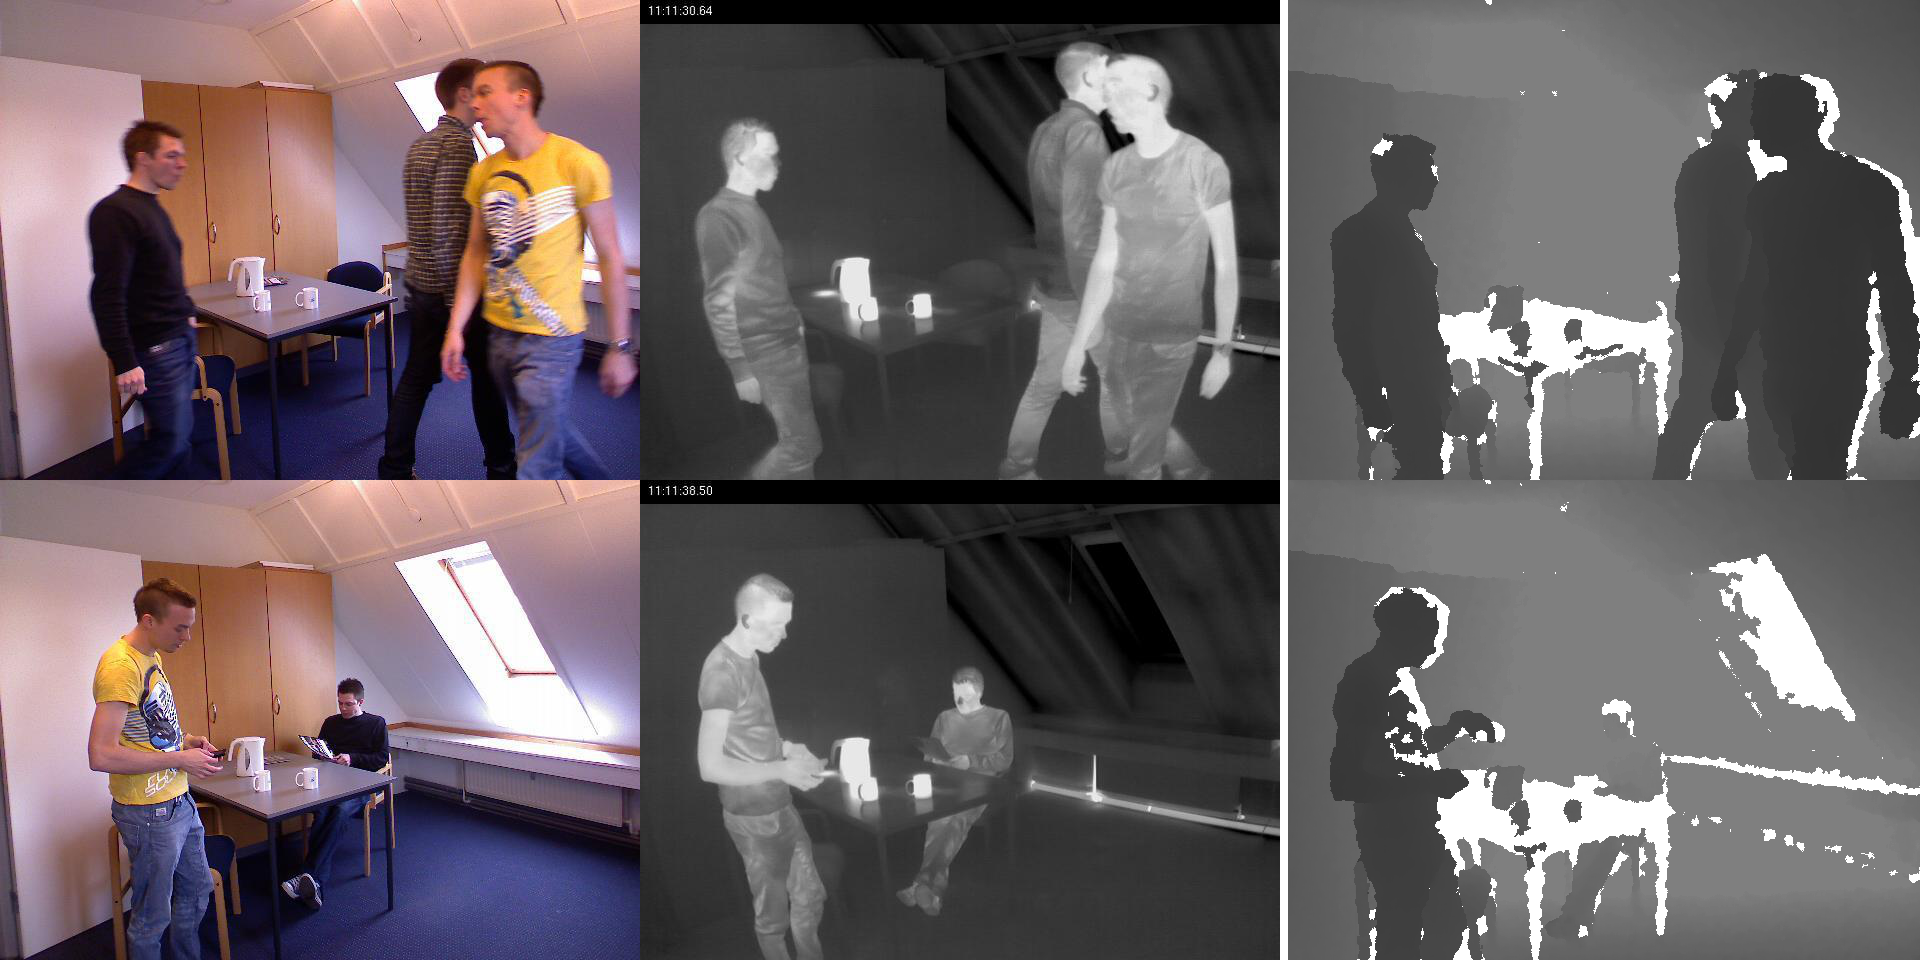
\includegraphics[width=0.48\textwidth]{Selection/1.png}
		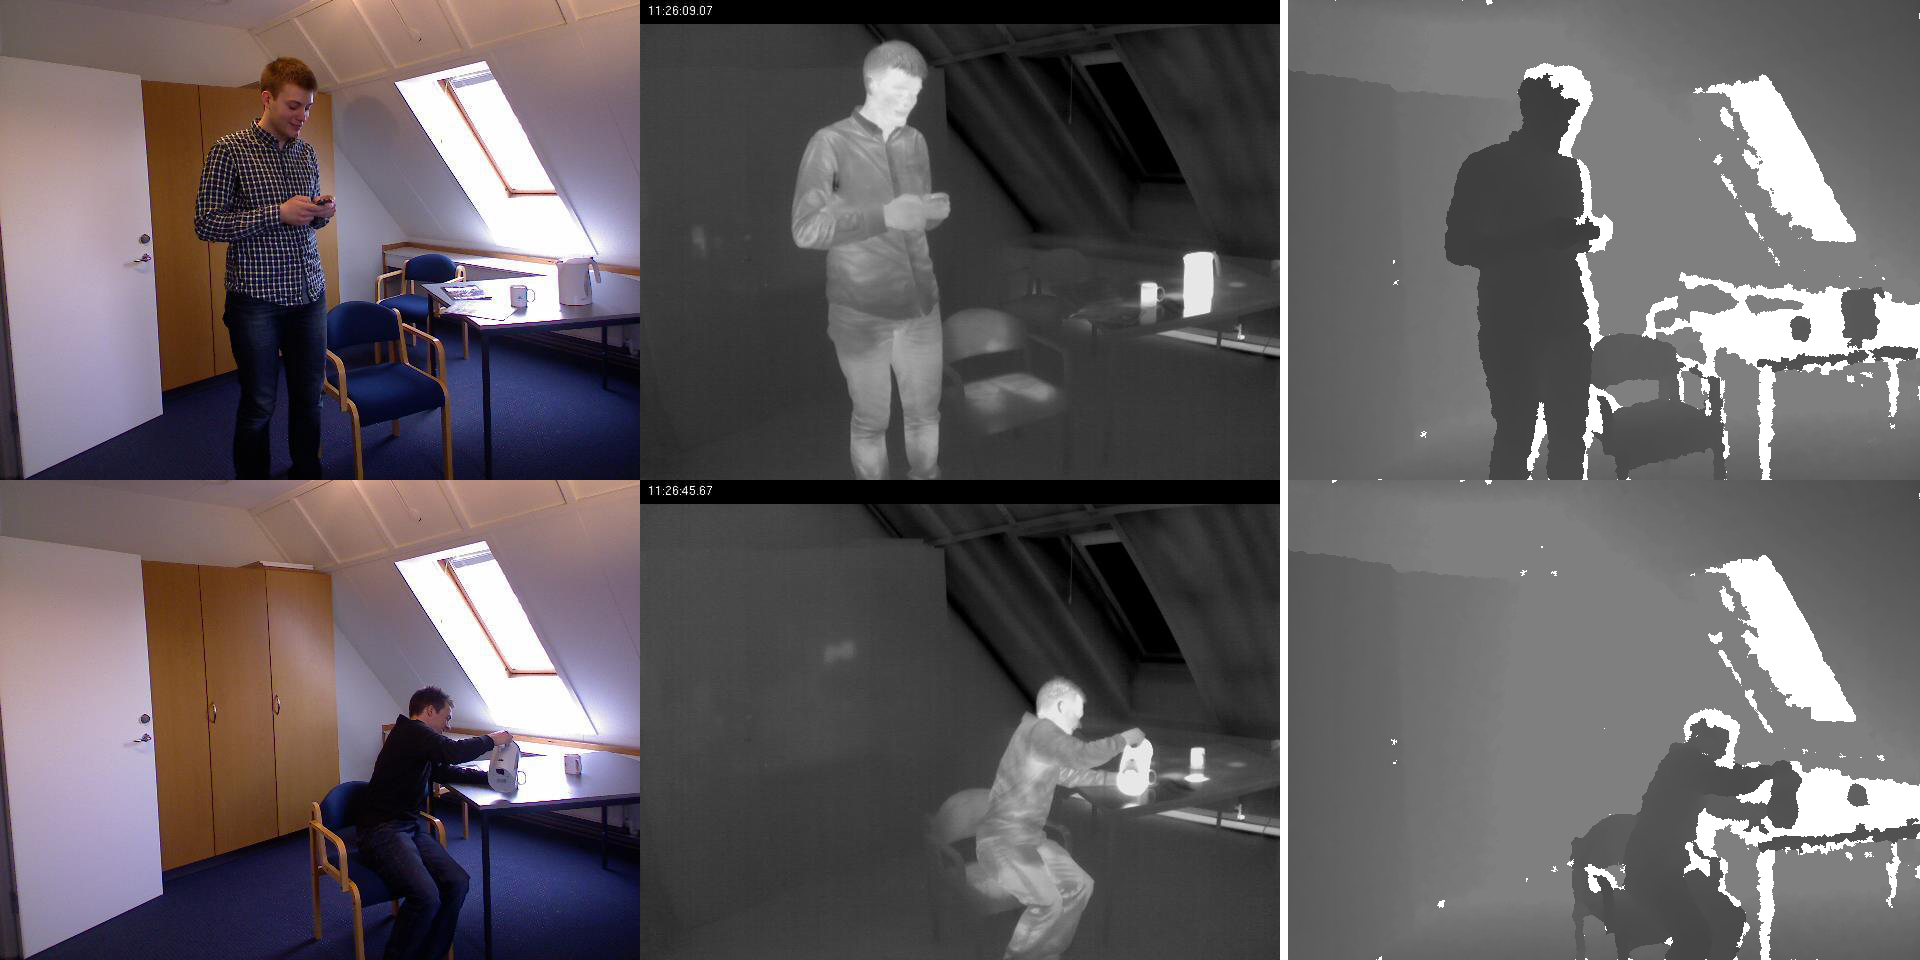
\includegraphics[width=0.48\textwidth]{Selection/2.png}
		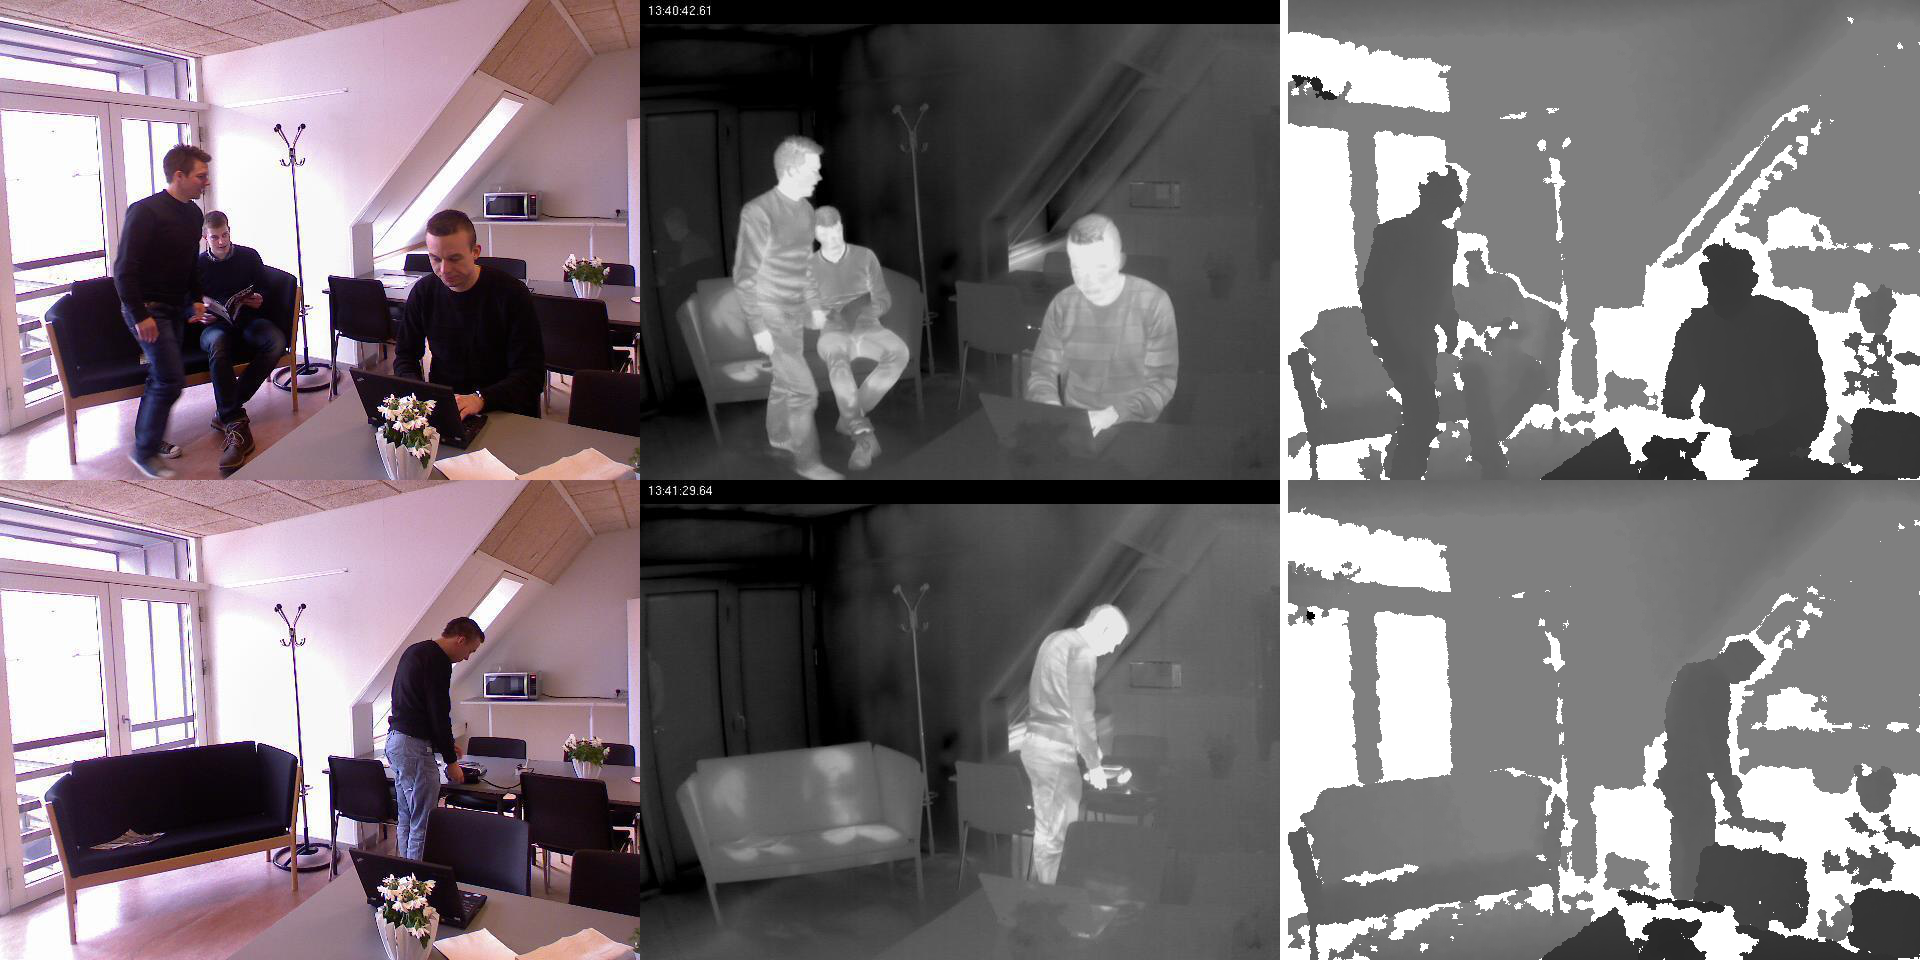
\includegraphics[width=0.48\textwidth]{Selection/3.png}
	\caption{Two views of each of the three scenes shown in the RGB, thermal, and depth modalities, respectively.}
	\label{fig:samplescenes}
\end{figure}

\begin{table}[htpb]
\centering
\begin{tabular}{llll}
\hline
Scene & Frames 	& Annotated frames 	& Depth range \\ \hline
1 		& 4693		& 1767	 						& 1-4 m \\
2 		& 2216		& 2016	 						& 1.4-1.9 m \\
3 		& 4628		& 1941	 						& 1-4 m \\ 
\hline
\end{tabular}
\caption{Annotated number of frames and spatial constraints of the scenes.}
\label{tab:scenes}
\end{table}

\subsection{Annotation}
%The frames are annotated using a pixel annotator tool ***ANDREAS TEXT HERE****
%
 %For each scene, human objects are annotated in the RGB modality. Each person is given a unique ID which he maintains throughout the scene. To obtain the corresponding masks in the thermal and depth modalities, the RGB masks are mapped using the registration algorithm of Section \ref{sec:registration}.
The acquired video was manually annotated frame-by-frame in a custom annotation program called Pixel Annotator. The dataset contains a large number of frames divided over a number of different sequences. All sequences have three modalities: RGB, depth, and thermal. The focus of the annotation has been on the persons in the scene and a mask-based annotation philosophy has been employed. That means that each person is covered by a mask and each mask (person) has a unique ID, which is consistent over frames. In this way the dataset can be used not only for background subtraction, but also for tracking and re-identification purposes. Since the main purpose of the dataset is background subtraction, a pixel-level annotation scheme was necessary - bounding boxes would not be sufficient.
 
As seen from Figure \ref{fig:pixelannotator}, Pixel Annotator provides a view of each modality with the current mask overlaid, as well as a raw view of the mask. It implements the registration algorithm described above so that the annotator can judge whether the mask fits in all modalities. Because the modalities are registered to each other, there is not specific masks for each modality, but a single mask for all.

\begin{figure}%
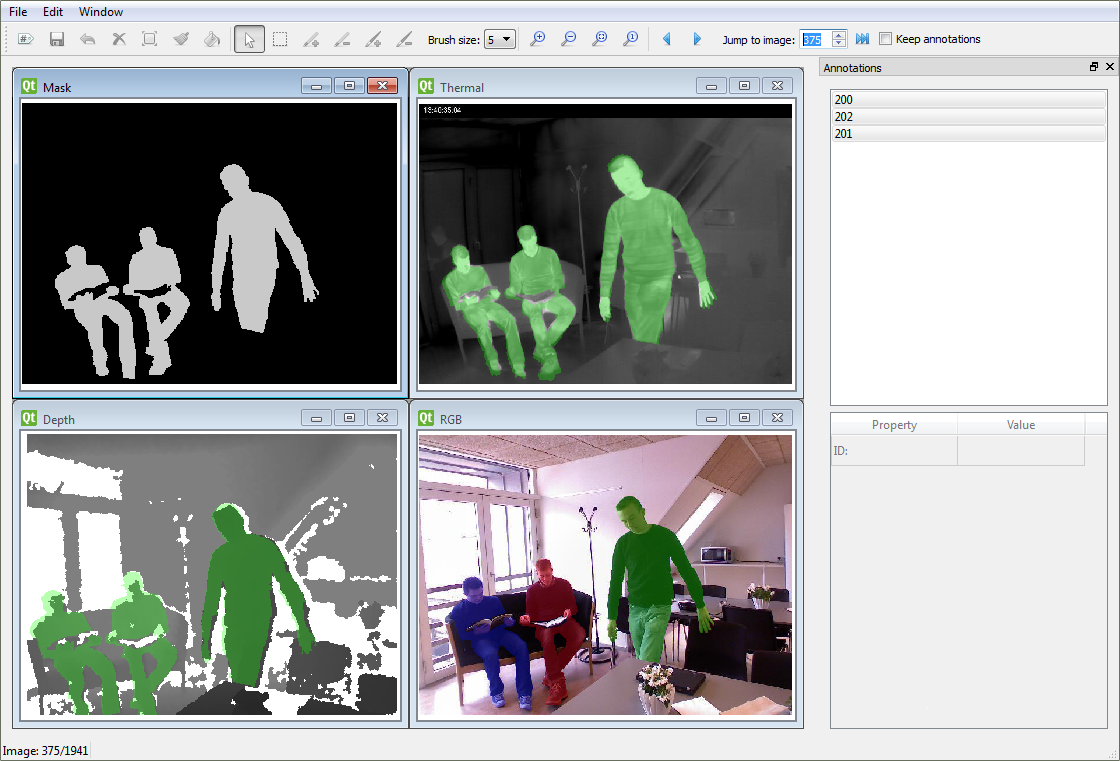
\includegraphics[width=0.48\textwidth]{pixelannotator2.png}%
\caption{Pixel Annotator showing the RGB masks and the corresponding, registered masks in the other views.}%
\label{fig:pixelannotator}%
\end{figure}

Each annotation can be initialized with an automatic segmentation using the GrabCut algorithm \cite{rother2004grabcut} to get quickly off the ground. Then Pixel Annotator provides pixel-wise editing functions to further refine the mask. Each annotation is associated with a numerical ID, and can have an arbitrary number of property fields associated with it. They can be boolean or contain strings, so advanced annotation can take place, all the way from simple occluded/not occluded fields to fields describing the current activity. Pixel Annotator is written in C++ on the Qt framework and is fully cross-platform compatible.

The data set and the registration algorithm is freely available at \cite{vapgroup}.

{\small
\bibliographystyle{ieee}
\bibliography{references}
}

\end{document}
